\documentclass[11pt,letterpaper,notitlepage]{article}

% Codificacion Windows
%\usepackage[latin1]{inputenc}
%\usepackage[spanish]{babel}

% Codificación GNU/Linux
\usepackage[utf8]{inputenc}
\usepackage[activeacute,spanish,es-tabla]{babel}

% Margenes
\usepackage{anysize}
\marginsize{2cm}{2cm}{2cm}{2cm}

% Estilo de pagina
\usepackage{fancyhdr}
\pagestyle{fancy}
\fancyhead[l]{\small EL5004 - Taller de Diseño}
\fancyhead[r]{
\includegraphics[scale=0.5]{fcfm}}

% Simbolos y letras para matemáticas
\usepackage{amssymb,amsmath,amsfonts}

% Colores
\usepackage{color}
\definecolor{rojo}{RGB}{255,26,34}
\definecolor{gris}{RGB}{104,108,113}
\definecolor{mygreen}{RGB}{28,172,0} % color values Red, Green, Blue
\definecolor{mylilas}{RGB}{170,55,241}

% Elementos Flotantes (Figuras y Tablas)

\usepackage{graphicx}
\graphicspath{ {img/} }
\usepackage{caption}
\usepackage{subcaption}
\usepackage{float}
\usepackage[binary-units=true]{siunitx}
\usepackage{multicol}
\usepackage{multirow}
\usepackage{epstopdf}
\usepackage{enumerate}
\usepackage{wrapfig}
\usepackage{enumitem}
\usepackage{hyperref}
\usepackage[numbered,framed]{mcode} %Código MATLAB
\hypersetup{
    colorlinks,
    linkcolor={gris},
    citecolor={gris},
    urlcolor={gris}
}
%Codigo fuente

\usepackage{listings}
\setlength{\headheight}{30pt} 


% Linea
\newcommand{\HRule}{\rule{\linewidth}{.4mm}}
\renewcommand{\lstlistingname}{Código fuente}
\renewcommand{\lstlistlistingname}{Indice de códigos fuente}

\newcommand{\portada}[3]{

\begin{titlepage}

%Encabezado
\begin{wrapfigure}{l}{.6cm}
\vspace{-0.65cm}

\includegraphics[width=4cm]{fcfm}
\end{wrapfigure}
\hspace*{0.3cm}
\textsc{\color{rojo}\hspace{2.2cm}Departamento de Ingeniería Eléctrica}\\
\hspace*{0.3cm}
\textsc{\color{gris}\hspace{2.8cm}Facultad de Ciencias Físicas y Matemáticas}\\
\hspace*{0.3cm}
\textsc{\color{gris}\hspace{2.8cm}Universidad de Chile}\\
\hspace*{0.3cm}
\textsc{\color{gris}\hspace{2.8cm}EL5004 - Taller de Diseño}\\


% Titulo
\begin{center}
~\\[4.5cm]
{\color{gris} \Large \textbf{#2}}
\HRule~ \\[0.8cm]
{ \Huge \textup \bfseries  #1}\\[0.4cm]
\HRule ~\\[1.5cm]
\end{center}
\begin{minipage}{.5\textwidth}
~
\end{minipage}
%Datos
\begin{minipage}{.5\textwidth}
\begin{flushright}
\begin{tabular}{l}
\emph{Profesor:} \\
{\small Marcos Orchard}\\[0.3cm]
\emph{Profesores Auxiliares:} \\
{\small Alejandro Toledo}\\
{\small Isao Parra}\\[0.3cm]
\emph{Estudiantes:}\\
{\small Matías Godoy}\\
{\small David Gómez}\\
{\small Eduardo Hormazábal}\\
{\small Rodrigo Muñoz}\\
{\small Sebastián Piña}\\
{\small Matías Silva}\\
{\small Yoshiro Tsutsumi}\\[.3cm]
\emph{Fecha:}\\
{\small \today}
\end{tabular}
\end{flushright}
\end{minipage}

\end{titlepage}
}

\begin{document}

\portada{Diseño de actuación y teleoperación de vehículo tipo Gokart}{Informe de Avance}

\newpage
\thispagestyle{empty}
\tableofcontents
\newpage

\vspace*{-0.8cm}

\section{Introducción}

Este trabajo se enmarca dentro del contexto del curso EL5004 Taller de Diseño, en el que se lleva a cabo un proyecto multidisciplinario entre estudiantes de ingeniería mecánica e ingeniería eléctrica, con el fin de lograr el acercamiento entre ambas disciplinas y el aprendizaje que esto conlleva, no solo de trabajo en equipo sino de acercar a los estudiantes a lo que corresponde a un proyecto real junto a todas sus partes: concebir, diseñar, implementar y operar.
En este caso, se propone desarrollar una teleoperación de un vehículo tipo goKart construido por alumnos del departamento de ingeniería mecánica. Esto es, comandar a distancia las acciones de giro, aceleración y freno de este vehículo. Para ello se debe realizar un diseño mecánico para el montaje de los nuevos mecanismos, como así un diseño eléctrico de la conexión y comunicación entre los actuadores. 


\section{Diseño mecánico}

En esta sección se muestran los distintos elementos mecánicos desarrollados, se muestran los requerimientos, los mecanismos involucrados y la solución implementada de cada uno de los actuadores.

%%%%%% DIRECCION %%%%%%
\subsection{Dirección}

\subsubsection{Requerimientos}

Se requiere un sistema de actuación sobre el giro del goKart, el cual logre los \SI{60}{\degree} de movilidad que se tienen (30° tanto para izquierda como derecha, con respecto al centro). Además, debe cumplir los requerimientos de torque los cuales se midieron en condiciones estáticas con el fin de sobredimensionar lo requerido, obteniendo con ello un factor de seguridad. Los requerimientos se resumen en la Tabla \ref{sw} . El brazo para el torque corresponde a la distancia entre centro del volante y extremos (\SI{10}{\centi\meter}). 

\begin{table}[H]
\centering
\begin{tabular}{l|l|l|}
\cline{2-3}
                                & Torque \si{\newton\meter} & Ángulo giro \si{\degree} \\ \hline
\multicolumn{1}{|l|}{Derecha}   & 12,75                     & 30                       \\ \hline
\multicolumn{1}{|l|}{Izquierda} & 8,83                      & 30                       \\ \hline
\end{tabular}
\caption{Tabla de requerimientos para actuar dirección.}
\label{sw}
\end{table}

\subsubsection{Propuesta}

Se propone una sistema de engranes rectos acoplados tanto al eje de dirección como al motor utilizado. Este último corresponde a la serie Dynamixel EX-106+, que entrega un torque máximo de \SI{10.4}{\newton\meter} y un ángulo de giro de \SI{250}{\degree}, así que dado los requerimientos (\SI{60}{\degree}), se estable una relación de 3:1 en el sistema de engranes, con el fin de utilizar toda la resolución del encoder del motor. Por otro lado, esto permite no forzar al motor a su torque máximo, sino a un tercio de su capacidad, quedando sobredimensionado ante cualquier falla que ocurra (factor de seguridad de 2.5 entre torque máximo y torque exigido al motor).

Por recomendación, se nos sugirió usar engranes módulo 2, por lo que todos los cálculos para estos se basan en ese supuesto. En la Tabla \ref{engrane} se muestra un resumen de los parámetros de ambos engranes. La Figura \ref{eng} muestra un modelo de como quedaría el montaje. La plataforma que se construye para el motor considera el ángulo necesario para que ambos engranes queden alineados. Se diferencia entre una plancha fija (color gris) y una plancha roja (móvil). A este última va apernado el motor. El hecho de que sea móvil permite subir y bajar el engrane del motor para ajustar los dientes de este con los del otro engranaje. La fijación se realiza con pernos Parker de cabeza plana.

El engrane de dirección consta de un acople de \SI{65}{\milli\meter} de diámetro y 20 mm de ancho, el cual se usará para unirlo al eje de dirección mediante un pasador partido de 6 mm de diámetro. Además cuenta con una perforación central de 10 mm de diámetro que corresponde al diámetro del eje. 

%@TODO
%Para mayores detalles de medidas, revisar anexo.  

\begin{table}
\centering


\begin{tabular}{l|l|l|}
\cline{2-3}
                                          & Engrane motor & Engrane dirección \\ \hline
\multicolumn{1}{|l|}{Módulo}              & 2             & 2                 \\ \hline
\multicolumn{1}{|l|}{Diámetro exterior \si{\milli\meter}} & 46      &  136    \\ \hline
\multicolumn{1}{|l|}{Paso}                & 6.28          & 6.28              \\ \hline
\multicolumn{1}{|l|}{Número Dientes}      & 21            & 66                \\ \hline
\multicolumn{1}{|l|}{Altura cabeza de diente \si{\milli\meter}} & 4.32  & 4.32\\ \hline
\multicolumn{1}{|l|}{Ancho de engranes \si{\milli\meter}} & 10 & 10            \\ \hline
\end{tabular}
\caption{Parámetros de engranes}
\label{engrane}
\end{table}

\begin{figure}[H]
\begin{center}
    \begin{subfigure}{0.4\textwidth}
        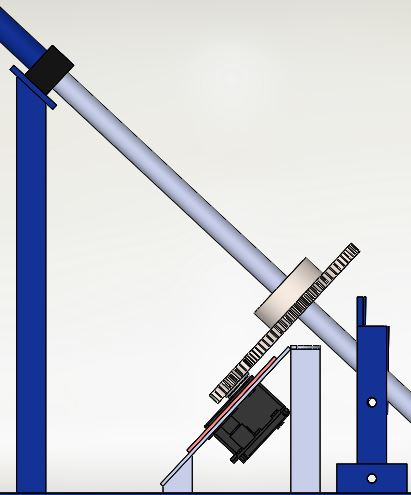
\includegraphics[width=0.9\linewidth, height=5cm]{diseno_mecanico/direccion/sw1.JPG} 
        \label{sw11}
    \end{subfigure}
    \begin{subfigure}{0.4\textwidth}
        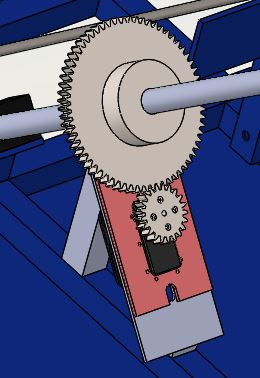
\includegraphics[width=0.9\linewidth, height=5cm]{diseno_mecanico/direccion/sw2.JPG}
        \label{sw22}
    \end{subfigure}
    \caption{Diseño CAD del actuador de dirección}
    \label{eng}
\end{center}
\end{figure}

\subsubsection{Resultados}

La Figura \ref{engraneFinal} muestra el montaje final. En la plataforma del motor se incluyó una pieza rectangular que une a ambos pilares con el fin de utilizar pernos para el montaje en el chasis del auto. El engrane de dirección no tiene todo los dientes puesto que solo rota en \SI{60}{\degree}, por lo que se dentó un cuarto (\SI{90}{\degree}) del total. El acople de este mismo se disminuyo para reducir peso, quedando con \SI{15}{\milli\meter} de ancho. La posición de todo el montaje no quedó exactamente donde indica el CAD, dado que el escaso espacio dificultaba el montaje, por lo que se corrió hacia el otro extremo (el engrane de dirección se subió a lo largo del eje) y se ajustó el engrane del motor usando la plataforma móvil su máxima altura, con el fin de que los dientes de ambos engranen quedaran bien acoplados. Se tuvo que devastar los soporte plásticos negros que mantienen el eje de dirección (se ven en la figura \ref{eng}) para así acercar más la dirección (y el engrane) al motor.

Dado que el diseño del goKart contempla movilidad de su dirección a lo largo (el volante se puede hundir o acercar al usuario), se pueden desacoplar los engranes, en el caso que se quiera manejar de manera manual el auto. Esto conlleva el problema de que los dientes de ambos engranes no están fijos, pues la vibración propia del auto al estar encendido hace que la dirección vibre a su vez y los dientes se muevan un poco entre sí, sin desacoplarse. A futuro se propone fijar la dirección en una posición (volante fijo) tal que el sistema de engrane no se altere.

\begin{figure}[H]
\begin{center}
    \begin{subfigure}{0.4\textwidth}
        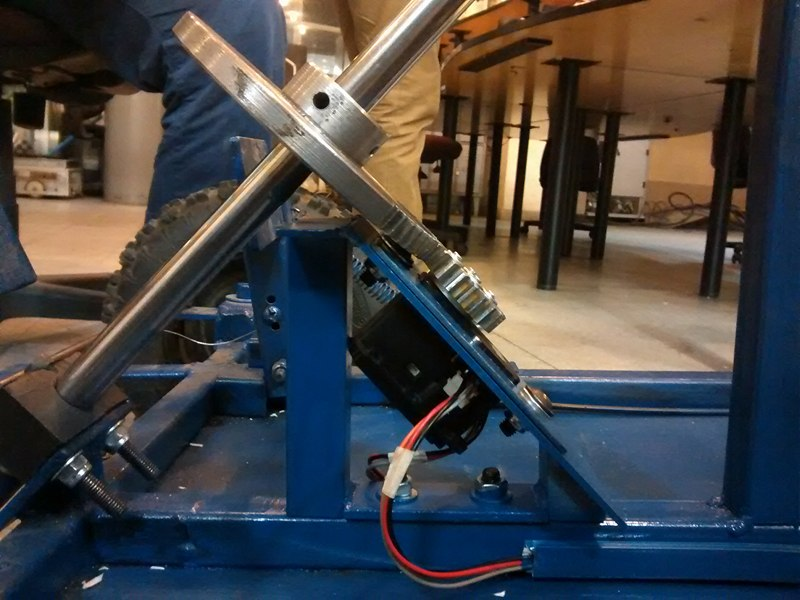
\includegraphics[width=0.9\linewidth, height=5cm]{diseno_mecanico/direccion/engrane1.jpg} 
        \label{sw1}
    \end{subfigure}
    \begin{subfigure}{0.4\textwidth}
        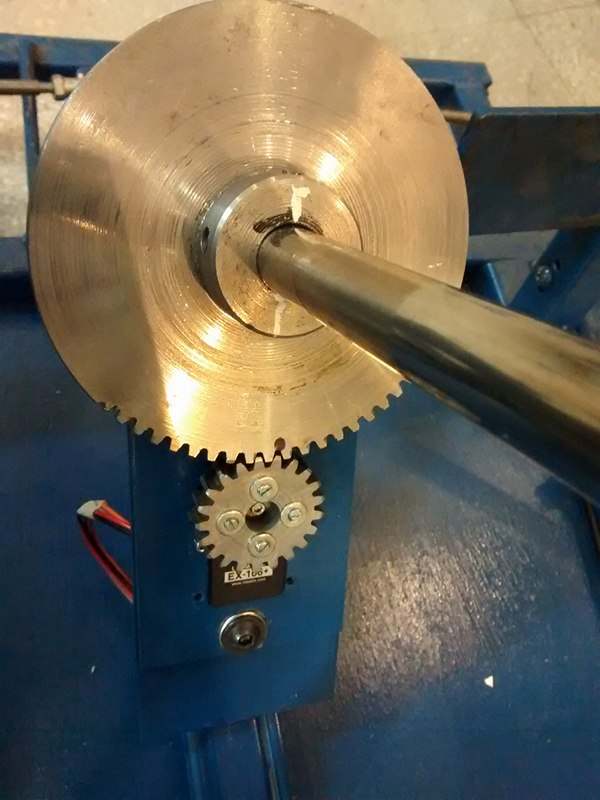
\includegraphics[width=0.9\linewidth, height=5cm]{diseno_mecanico/direccion/engrane2.jpg}
        \label{sw2}
    \end{subfigure}
    \caption{Implementación del actuador de dirección}
    \label{engraneFinal}
\end{center}
\end{figure}


%%%%%% FRENO %%%%%%
\subsection{Freno}

\subsubsection{Requerimientos}
La implementación de este sistema tiene por objetivo actuar eléctricamente sobre el freno sin comprometer al sistema manual del vehículo, es decir un sistema de frenado mixto. Esto implica que si se acciona el frenado eléctricamente, el piloto tenga la posibilidad de usar el freno manual en todo momento, y viceversa.

El sistema manual consiste en un freno hidráulico accionado por un pistón conectado a una vara móvil con la que se comprime el líquido en su interior (Figura \ref{piston}).

\begin{figure}[H]
\begin{center}
	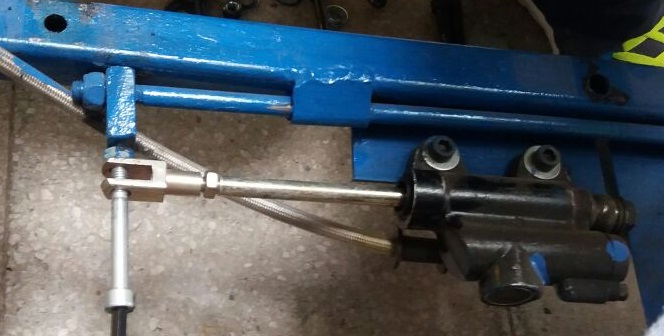
\includegraphics[width=0.5\textwidth]{diseno_mecanico/freno/piston.jpg}
	\caption{Pistón del sistema de freno del vehículo.}
	\label{piston}
\end{center}
\end{figure}


\subsubsection{Propuesta}

La solución propuesta consiste en añadir una pieza móvil (Figura \ref{cad_roldana}, pieza naranja) denominada roldana, que accione el freno hidráulico del sistema original mediante un adaptador que otorgue el desacoplamiento de ambos sistemas (Figura \ref{cad_roldana}, pieza gris). Cabe destacar que el adaptador sustituye a la pieza que empuja al pistón de la Figura \ref{piston}. El movimiento mecánico lo accionará un servomotor Dynamixel EX-106+ \cite{motor_datasheet}.

\begin{figure}[H]
\begin{center}
	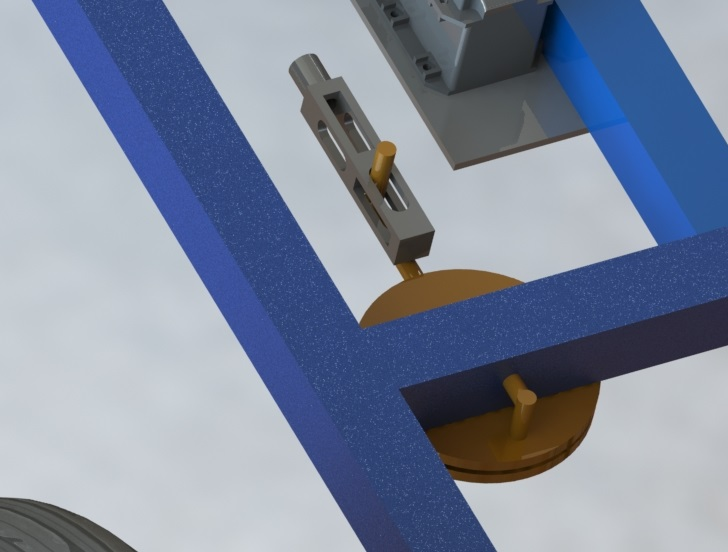
\includegraphics[width=0.5\textwidth]{diseno_mecanico/freno/render_freno3.jpg}
	\caption{CAD roldana y adaptador del freno.}
	\label{cad_roldana}
\end{center}
\end{figure}

El objetivo es que la roldana empuje el adaptador al accionar el servomotor. Para ello se propone que uno de los extremos de la guía de la roldana esté fijo, mientras el otro se conecte al disco de giro del servomotor. De esta forma, al accionar el motor, variará la longitud efectiva de la guía y con ello la posición de la roldana. En particular se midió que la retracción necesaria que se le debe aplicar al pistón para un frenado completo es de 15 mm, por lo que la guía debería reducir su longitud efectiva en 30 mm (asumiendo simetría de la guía con respecto al eje de movimiento de la roldana).

Con el fin de generar el menor roce posible para el movimiento de la roldana se determinó que la guía de ésta estuviera paralela al eje de movimiento, restringiendo las posibles ubicaciones del servomotor. En la Figura \ref{cad_freno} se muestra la posición del servomotor y del chasis añadido que lo sostiene. También se observan las tres piezas sostenedoras de la roldana: una superior atravesando horizontalmente el chasis, y dos pernos inferiores por los que se mueve la roldana.

\begin{figure}[H]
\begin{center}
    \begin{subfigure}{0.4\textwidth}
        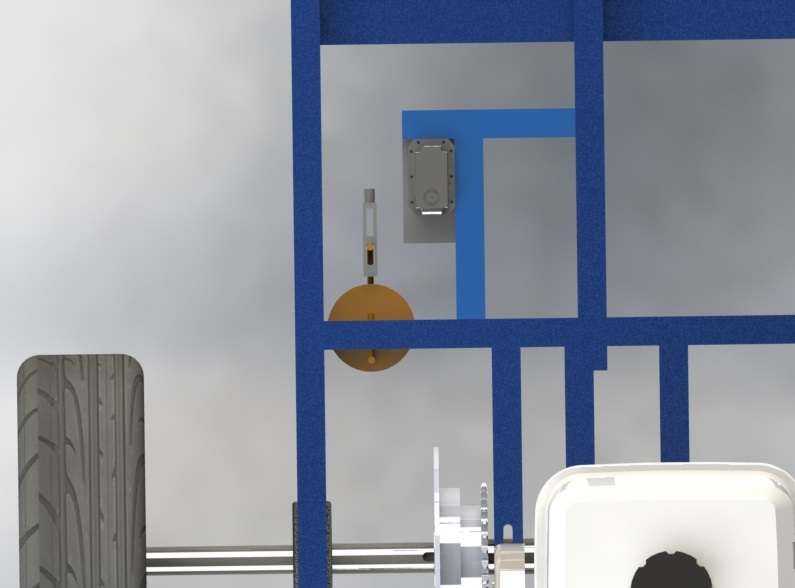
\includegraphics[width=0.9\linewidth, height=5cm]{diseno_mecanico/freno/render_freno1.jpg} 
        \label{freno1}
    \end{subfigure}
    \begin{subfigure}{0.4\textwidth}
        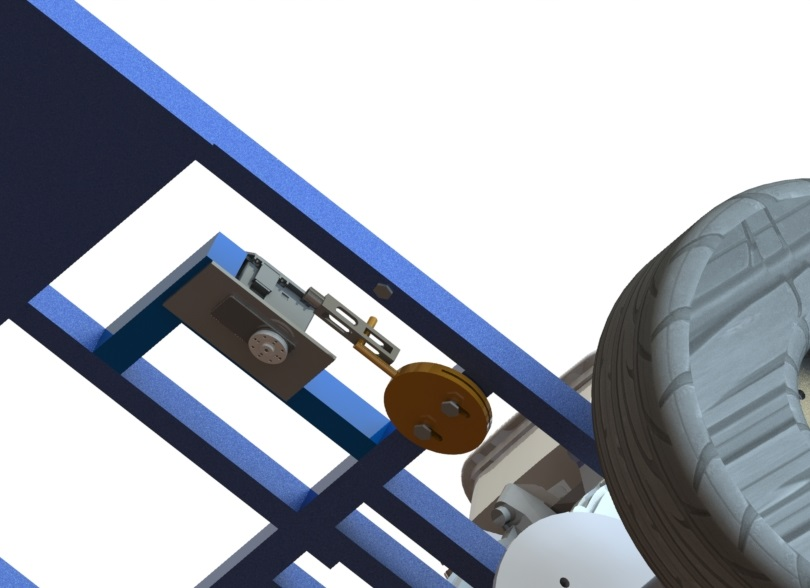
\includegraphics[width=0.9\linewidth, height=5cm]{diseno_mecanico/freno/render_freno2.jpg}
        \label{freno2}
    \end{subfigure}
    \caption{Diseño CAD del actuador del freno.}
    \label{cad_freno}
\end{center}
\end{figure}


\subsubsection{Resultados}

Las piezas principales del sistema (roldana y adaptador) resultaron de la forma esperada. No obstante, se realizaron ligeros cambios con respecto al montaje de la roldana, pues solamente se implementaron dos de las tres piezas sostenedoras (los pernos) debido al limitado espacio disponible entre la roldana y el disco de freno (Figura \ref{res_freno}).

En la Figura \ref{res_freno} se muestran tres estados distintos del sistema de frenado mixto. La Figura \ref{res_freno1} muestra el estado de reposo, es decir que el vehículo no está frenado. En la Figura \ref{res_freno2} se observa el desplazamiento de la roldana debido al accionamiento del servomotor, causando el frenado del goKart sin necesidad de actuar en el freno manual. La Figura \ref{res_freno3} indica un frenado manual sin movimiento del servomotor por lo que la roldana permanece en la posición de reposo y la guía se destensa levemente, pero no lo suficiente como para desprenderse de la roldana. En el caso de un frenado simultáneo (manual y eléctrico) se produce un resultado similar al frenado manual, con la diferencia de que la roldana se desplaza y la guía permanece tensa.



\begin{figure}[H]
\begin{center}
    \begin{subfigure}{0.3\textwidth}
        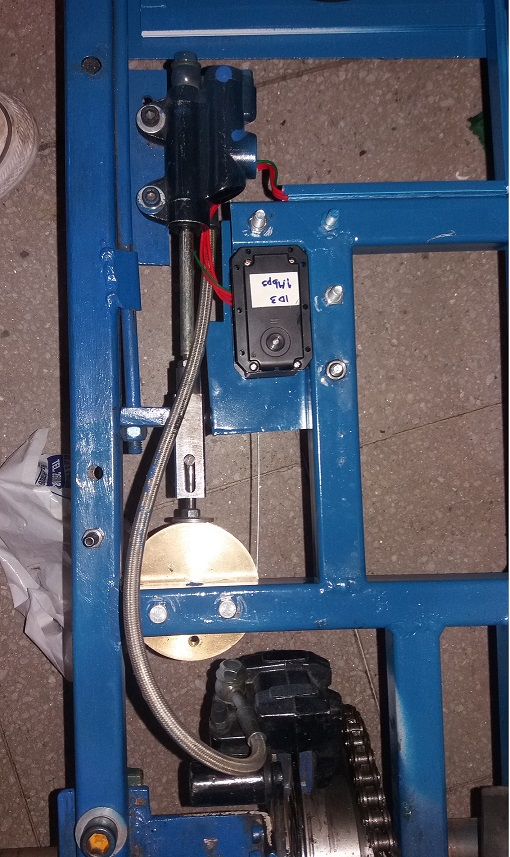
\includegraphics[width=1\linewidth, height=9cm]{diseno_mecanico/freno/no_freno.jpg} 
        \caption{Sistema en reposo.}
        \label{res_freno1}
    \end{subfigure}
    \begin{subfigure}{0.3\textwidth}
        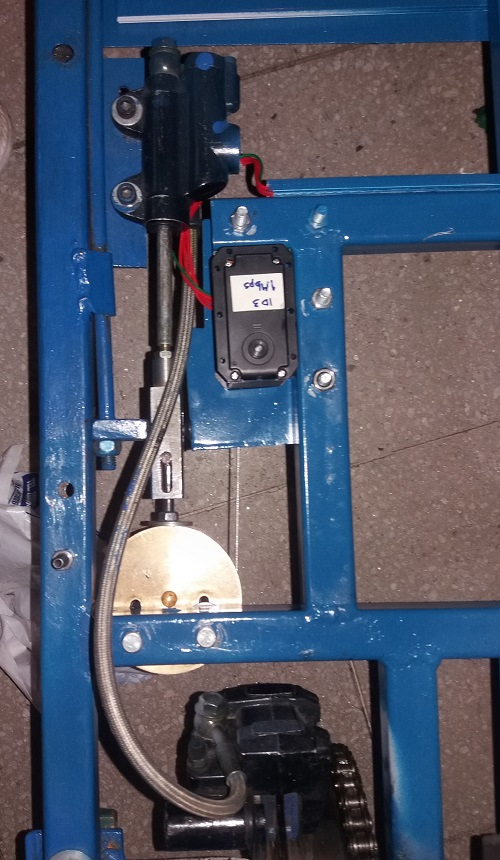
\includegraphics[width=1\linewidth, height=9cm]{diseno_mecanico/freno/freno_motor.jpg}
        \caption{Freno accionado por motor.}
        \label{res_freno2}
    \end{subfigure}
    \begin{subfigure}{0.3\textwidth}
        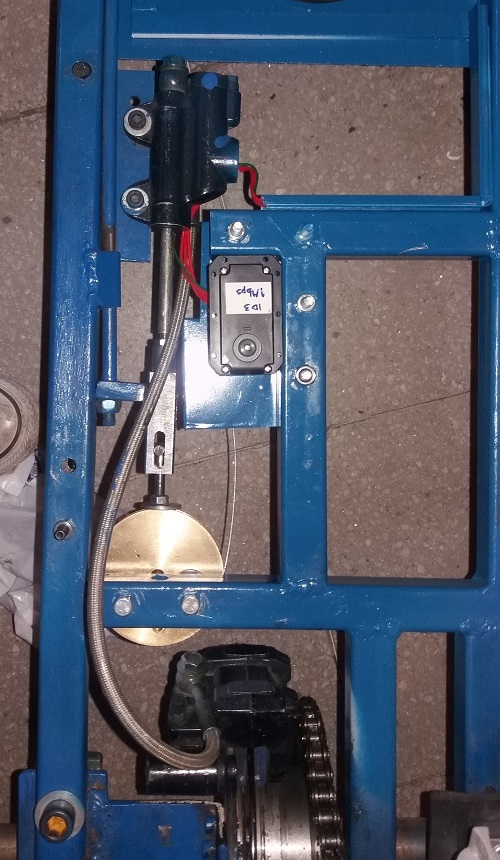
\includegraphics[width=1\linewidth, height=9cm]{diseno_mecanico/freno/freno_manual.jpg}
        \caption{Freno accionado manualmente.}
        \label{res_freno3}
    \end{subfigure}
    \caption{Actuador del freno en sus estados principales.}
    \label{res_freno}
\end{center}
\end{figure}





%%%%%% ACELERADOR %%%%%%
\subsection{Acelerador}

\subsubsection{Requerimientos}

De la misma forma que el frenado, la implementación de este sistema tiene por objetivo actuar eléctricamente sobre el acelerador sin comprometer al sistema manual del vehículo, es decir un sistema de aceleración mixto. Esto implica que el acelerador se pueda accionar tanto eléctrico como manualmente. 
El sistema manual consiste en una piola conectada directamente al pedal de aceleración; y en su otro extremo, al acelerador del motor del goKart.


\subsubsection{Propuesta}
Se propone incluir una pieza intermediaria entre los actuadores y la piola conectada al acelerador del motor. La pieza corresponde a una platina de acero móvil a través de unos ejes (Figura \ref{platina}), en donde por un extremo se conecta la piola del acelerador, y por el otro se encajan las piolas de los sistemas manual y eléctrico. El actuador eléctrico corresponde a un servomotor Dynamixel ex-106+ \cite{motor_datasheet}.

\begin{figure}[H]
\begin{center}
	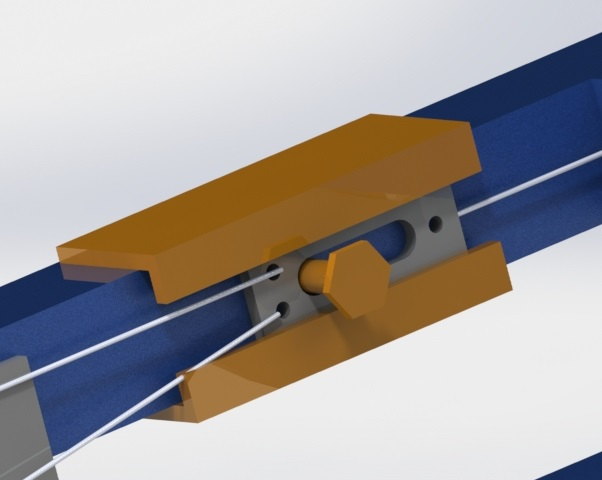
\includegraphics[width=0.4\textwidth]{diseno_mecanico/acelerador/render_acelerador2.jpg}
	\caption{CAD de platina con los ejes como guía.}
	\label{platina}
\end{center}
\end{figure}

Las tres secciones de piola conectadas a la platina deben estar tensadas en el reposo, lo que causa el movimiento de la platina si se presiona el pedal del acelerador (sistema manual) o si se rota el disco de giro servomotor (sistema eléctrico) y por ende, se accionará el acelerador del motor del goKart (Figura \ref{cad_acelerador}). Esta propuesta parte de la premisa que las piolas pueden aflojarse cierta cantidad, pues al momento de activar un sistema de acelerador, la piola del otro quedará en desuso. Cabe destacar que el desplazamiento máximo de la piola para acelerar, en el sistema manual original, es de aproximadamente 3 cm.

\begin{figure}[H]
\begin{center}
	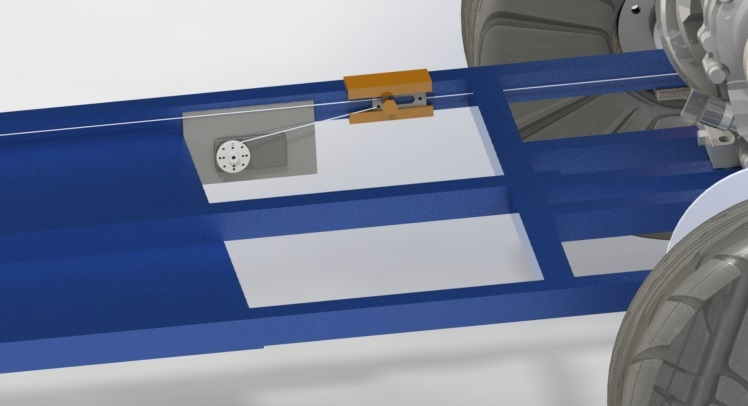
\includegraphics[width=0.5\textwidth]{diseno_mecanico/acelerador/render_acelerador1.jpg}
	\caption{Diseño CAD del actuador del acelerador.}
	\label{cad_acelerador}
\end{center}
\end{figure}

Como medida de seguridad se optó por ubicar un resorte en el extremo de la platina cercano al motor, de manera que el sistema tienda a detener la aceleración con la fuerza del resorte y no del sistema intrínseco del motor del goKart.


\subsubsection{Resultados}

La idea de deslizar una pieza por una guía se mantuvo, con la diferencia del tipo de piezas a utilizar. Finalmente se implementó un sistema con una corredera telescópica con rodamientos. Esto fue por el ínfimo roce que se opone al movimiento en comparación a una platina de acero.

Por otro lado, para generar holguras en las piolas y evitar fuerzas no deseadas por la piola en desuso cuando se active uno de los dos sistemas de aceleración, se optó por conectar las piolas a la corredera por medio de topes móviles (Figura \ref{res_acelerador}). La configuración en reposo consiste en tener las tres piolas tensas, y al momento de accionar un actuador la piola correspondiente jalará la corredera, mientras la otra estará en reposo, desacoplándose a la corredera.

En la Figura \ref{res_acelerador1} se muestra el estado en reposo, en donde las tres piolas se encuentran en una tensión que ocasiona que la corredera esté cercana al motor del goKart. La Figura \ref{res_acelerador2} indica una aceleración efectuada por el servomotor, de manera que la corredera se aleja del motor del goKart y la piola de sistema manual queda en un reposo parcial. Por último, en la Figura \ref{res_acelerador3} se tiene una aceleración manual, por lo que se obseva la corredera alejada del motor del vehículo, mientras que la piola del servomotor está en desuso.

\begin{figure}[H]
\begin{center}
    \begin{subfigure}{0.45\textwidth}
        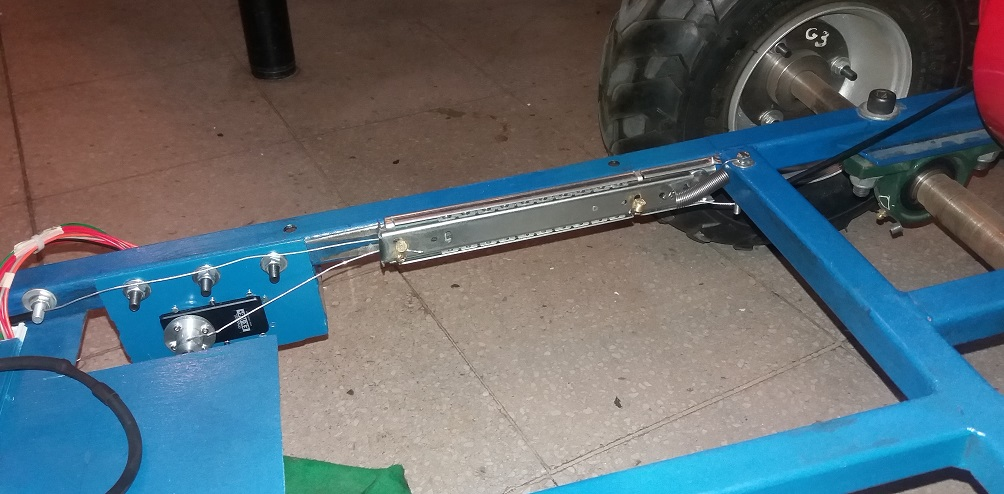
\includegraphics[width=1\linewidth]{diseno_mecanico/acelerador/no_aceleracion.jpg} 
        \caption{Sistema en reposo.}
        \label{res_acelerador1}
    \end{subfigure}
    \begin{subfigure}{0.45\textwidth}
        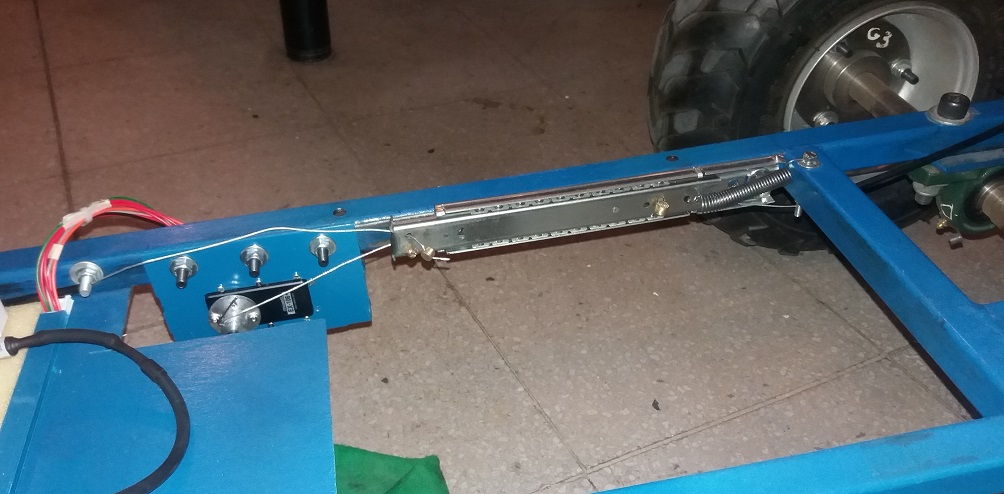
\includegraphics[width=1\linewidth]{diseno_mecanico/acelerador/aceleracion_motor.jpg}
        \caption{Sistema accionado por motor.}
        \label{res_acelerador2}
    \end{subfigure}
    
    \begin{subfigure}{0.45\textwidth}
        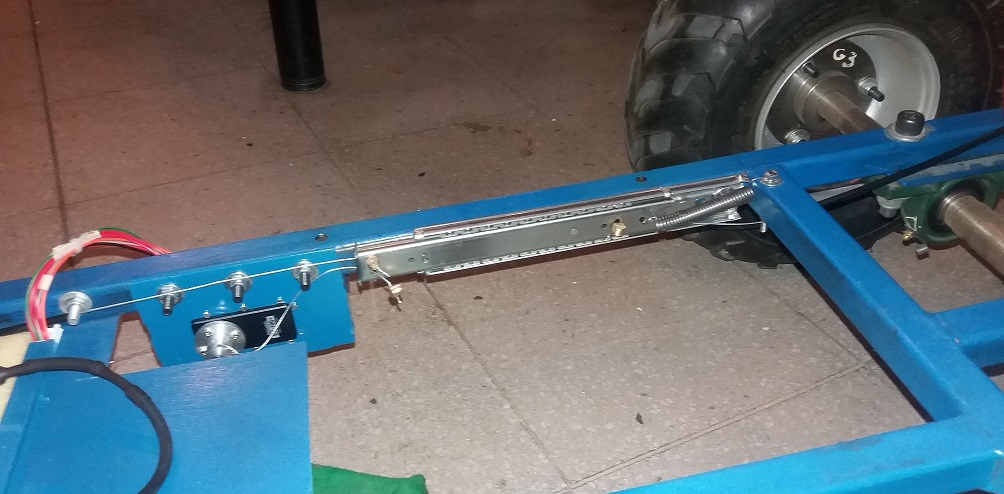
\includegraphics[width=1\linewidth]{diseno_mecanico/acelerador/aceleracion_manual.jpg}
        \caption{Sistema accionado manualmente.}
        \label{res_acelerador3}
    \end{subfigure}
    
    \caption{Actuador del acelerador en sus estados principales.}
    \label{res_acelerador}
\end{center}
\end{figure}

Por otro lado, en las imágenes de la Figura \ref{res_acelerador} se puede observar un resorte en el extremo de la corredera cercano al motor del goKart. Es el resorte de seguridad que se encarga de devolver la corredera al estado de reposo mientras ninguno de los sistemas de aceleración se activen.

\section{Diseño eléctrico}

En esta sección se muestran los distintos elementos del desarrollo en el plano eléctrico y electrónico.

\subsection{Diagrama eléctrico}

La Figura \ref{de_diagrama} muestra el diagrama eléctrico principal, este cuenta con los siguientes elementos:
\begin{itemize}
    \item \textbf{Batería}: La batería corresponde a un pack de 4 celdas de polímero de litio. Posee un voltaje nominal de \SI{14.8}{\volt} y una capacidad de \SI{3300}{\milli\ampere\hour}. Este tipo de baterías se caracterizan por su gran densidad energética y capacidad de descarga, por lo es óptima para la operación de motores, pues usualmente requieren peaks corriente del orden de \SI{5}{\ampere}.
    \item \textbf{Panel de control}: En su interior contiene el microcontrolador y receptor de radio.
    \item \textbf{Interruptor principal}: Es el encargado de conectar la batería con el resto de los circuitos.
    \item \textbf{Interruptor de emergencia}: Desconecta la energía del bus de actuadores Dynamixel, no interfiere con la alimentación del panel de control.
    \item \textbf{Bus Dynamixel}: Este bus esta constituido por cuatro conductores. Dos de ellos proporcionan alimentación a los dispositivos conectados ($V_{cc}$ y tierra). Los otros dos corresponden a la señal diferencial del bus RS485.
\end{itemize}

\begin{figure}[H]
\begin{center}
	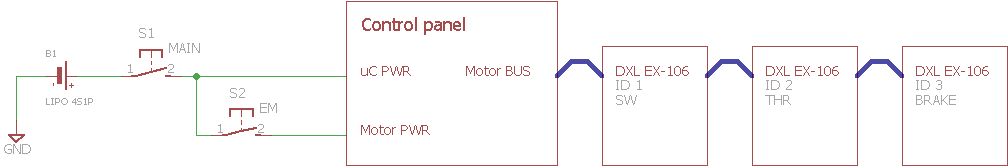
\includegraphics[width=0.9\textwidth]{diseno_electrico/diagram.png}
	\caption{Diagrama elétrico principal.}
	\label{de_diagrama}
\end{center}
\end{figure}

\subsection{Sistema de radio}

Para la comunicación con el GoKart a través de telecomandos se está utilizando un transmisor de radiofrecuencias llamado Fly-Sky modelo FS-T6, junto a un receptor de 6 canales a 2.4 GHz llamado Fly-Sky modelo FS-R6B (ver en Figura \ref{rf}).

\begin{figure}[H]
    \centering
    \begin{subfigure}[b]{0.3\textwidth}
        \centering
        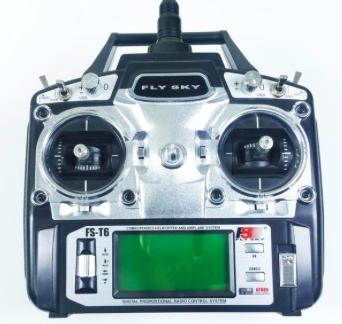
\includegraphics[width=0.9\textwidth]{diseno_electrico/rf_control.png}
        \caption{Control remoto}
        \label{rf_control}
    \end{subfigure}
    \begin{subfigure}[b]{0.3\textwidth}
        \centering
        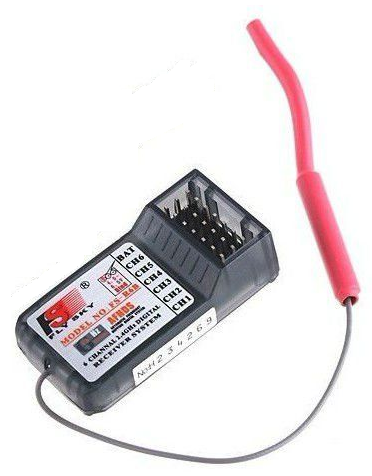
\includegraphics[width=0.9\textwidth]{diseno_electrico/rf.png}
	    \caption{Receptor de radio}
	    \label{rf_img}
    \end{subfigure}
    \caption{Hardware utilizado para telecomandar el gokart}\label{rf}
\end{figure}

De la radio transmisora se utilizarán 3 comandos:
\begin{enumerate}
    \item {\textbf{Manilla izquierda:} movimientos UP y DOWN para acelerar y frenar, respectivamente.}
    \item {\textbf{Manilla derecha: } movimientos LEFT y RIGHT para dirección.}
    \item {\textbf{Switch superior izquierda:} para activar estado de emergencia. }
\end{enumerate}

De esta forma, el receptor utiliza 3 de sus 6 canales para recibir los datos, los que resultan ser números enteros con un rango entre 1000-1400, que corresponden al valor en \si{\micro\second} del up-time de la señal PWM recibida.

\subsection{Sistema embebido}

El sistema cuenta con un microcontrolador principal encargado de recibir los comandos desde el receptor de radio y enviar comandos de movimiento a los servomotores. El sistema usa como elemento principal una placa de desarrollo Arduino Mega 2560 \cite{arduino_mega}, que se muestra en la Figura \ref{arduino_mega_img}. La Tabla \ref{arduino_mega_tab} muestra las principales características de la placa de desarrollo.

\begin{table}[H]
\centering
\begin{tabular}{|l|l|}
\hline
Microcontrolador        & ATmega2560                              \\ \hline
Voltaje de operación    & \SI{5}{\volt}                           \\ \hline
Limites de alimentación & \SI{6}{\volt} a \SI{20}{\volt}          \\ \hline
GPIO                    & 54                                      \\ \hline
Entradas ADC            & 16                                      \\ \hline
Memoria Flash           & \SI{256}{\kilo\byte}                    \\ \hline
SRAM                    & \SI{8}{\kilo\byte}                      \\ \hline
Velocidad de reloj      & \SI{16}{\mega\hertz}                    \\ \hline
Puertos UART            & 4                                       \\ \hline
\end{tabular}
\caption{Características Arduino Mega 2560}
\label{arduino_mega_tab}
\end{table}

\begin{figure}[H]
\begin{center}
	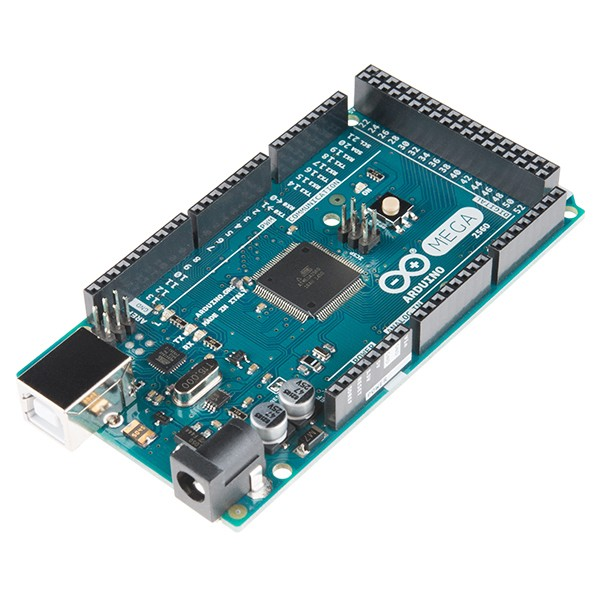
\includegraphics[width=0.3\textwidth]{diseno_electrico/arduino-mega.jpg}
	\caption{Arduino Mega 2560.}
	\label{arduino_mega_img}
\end{center}
\end{figure}

\subsubsection{Pantalla LCD}

La pantalla LCD empleada corresponde a LCD \textit{keypad shield} \cite{arduino_lcd}, esta placa es compatible con el extendido controlador Hitachi HD44780. La Figura \ref{arduino_lcd} muestra la placa utilizada.

\begin{figure}[H]
\begin{center}
	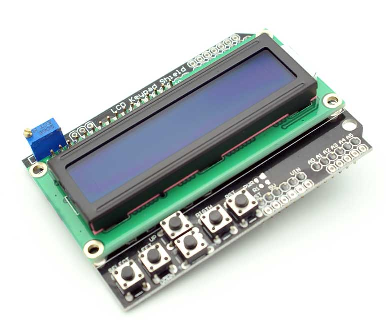
\includegraphics[width=0.5\textwidth]{diseno_electrico/lcd.png}
	\caption{LCD \textit{keypad shield} utilizado.}
	\label{arduino_lcd}
\end{center}
\end{figure}

\subsubsection{Interfaz con motores Dynamixel}

Los actuadores utilizados en este proyecto corresponden al modelo Dynamixel EX-106+ fabricados por Robotis. Estos actuadores son ampliamente utilizados en aplicaciones robóticas, integran su propio controlador, encoder, driver e interfaz de comunicación que permite la conexión de múltiples actuadores usando como capa física un bus RS485.

Para la conversión del puerto UART del del microcontrolador al estándar RS485 es necesario un \textit{transceiver}, en está aplicación se uso un integrado SN75176BP de Texas Instruments \cite{ic_rs485}.

Para la comunicación con los actuadores Dynamixel es necesario usar un protocolo especificado por el fabricante \cite{motor_datasheet}, dado la gran extensión de estos motores existen librerías que proveen una interfaz de software que implementan el protocolo.

\subsubsection{PCB}

Para el montaje del receptor de radio y componentes necesarios para la comunicación con los motores Dynamixel, se diseñó y construyó una PCB que se se empotra de forma natural a la placa Arduino Mega, pues se ha usado el formato conocido como \textit{shield}.

La Figura \ref{de_pcb} muestra el diseño de la PCB, donde se ha considerado las conexiones para el \textit{transceiver} RS485, una pantalla LCD y potenciómetros para hacer una interfaz de usuario.

\begin{figure}[H]
\begin{center}
	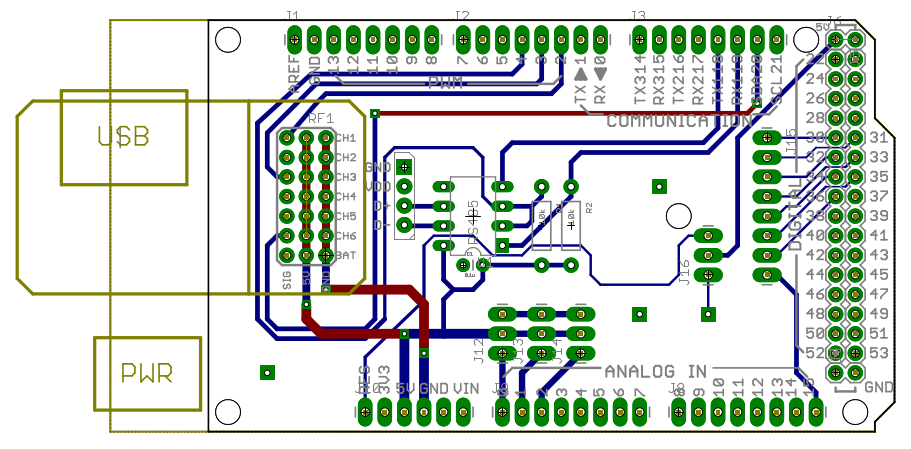
\includegraphics[width=0.5\textwidth]{diseno_electrico/pcb.png}
	\caption{PCB con formato \textit{shield}.}
	\label{de_pcb}
\end{center}
\end{figure}





\section{Software}
El software que ejecuta el microcontrolador para comunicar la radio transmisora y los actuadores en el auto se realizó utilizando un modelo de comunicación robusto, que garantizara el correcto funcionamiento del auto, activara rápidamente los casos de emergencia y ofreciera fácilmente una forma de comunicar la información al usuario del auto a través de una pantalla LCD (ver Sección 3.3).

Dado que el el \textit{toolchain} AVR GCC, usado para compilar el código para el microcontrolador, soporta el lenguaje C++, se hace en uso extensivo de programación orientada a objetos. Los elementos principales dentro del software (clases dentro del código) se detallan a continuación:
\begin{itemize}
    \item{\textbf{GoKartHW:}} Es el objeto principal o cerebro del código, al inicializarlo se inician los objetos que caracterizan los actuadores, la comunicación con el transmisor y con el LCD. También maneja el estado de emergencia, que implica detener frenar el auto y dejarlo con dirección hacia el centro.
    \item{\textbf{Dxl servo:}} Es el objeto encargado de la comunicación con los motores Dynamixel y configura los parámetros de velocidad, torque y posiciones mínimas y máximas que tienen actuadores. Estos objetos heredan de esta clase: 
    \begin{enumerate}
        \item{\textbf{Throttle:} Es el objeto que representa al actuador del acelerador y configura sus parámetros acorde a las características físicas de ese actuador en el montaje.}
        \item{\textbf{Brake:} Es el objeto que representa al actuador del freno y configura sus parámetros acorde a las características físicas de ese actuador en el montaje.}
        \item{\textbf{Steering Wheel:} Es el objeto que representa al actuador ligado al manubrio y configura sus parámetros acorde a las características físicas de ese actuador en el montaje.}
    \end{enumerate}
    
    \item{\textbf{RFInterface:} Es el objeto que controla el proceso de lectura de datos del receptor desde el transmisor RF. Este objeto recibe estos datos, los valida (según una configuración propia) y mapea hacia los actuadores. En caso de que los datos estén corruptos o no se estén recibiendo, entonces comanda al Gokart al estado de emergencia.}
    \item{\textbf{LCD:} Es el objeto que controla la pantalla LCD, su escritura y la forma en que se muestren y limpien los datos en la pantalla. Por tanto, a través de este objeto el Gokart envía los mensajes de los procesos que desee mostrar.}
\end{itemize}

Se ha hecho uso de herramientas de control de versiones e integración continua para el desarrollo de software de forma colaborativa. Esto permite que, de forma automatizada, cada aporte sea validado antes de su integración en el desarrollo principal.



\nocite{*}
\bibliographystyle{plain}
\bibliography{bibliografia}


\end{document}